%!TEX root = ../thesis_phd.tex
%%%%%%%%%%%%%%%%%%%%%%%%%%%%%%%%%%%%%%%%%%%%%%%%%%%%%%%%%%%%%%%%%%%%%%%%%%%%%%%%
% cnn.tex:
%%%%%%%%%%%%%%%%%%%%%%%%%%%%%%%%%%%%%%%%%%%%%%%%%%%%%%%%%%%%%%%%%%%%%%%%%%%%%%%%
\chapter{Convolutional Neural Network Event Classifier}
\label{cnn_chapter}
%%%%%%%%%%%%%%%%%%%%%%%%%%%%%%%%%%%%%%%%%%%%%%%%%%%%%%%%%%%%%%%%%%%%%%%%%%%%%%%%

At the core of any particle physics analysis is the selection of signal events,
that is, the events which represent the physical process under study.
Traditionally, features are extracted from event reconstruction and passed
to a machine learning alrorithm \cite{lecun2015deep}, e.g. k-nearest neighbor
\cite{altman1992introduction}, neural network \cite{reed1999neural},
or decision tree \cite{friedman2002stochastic}.
While this apporach is generally successful, those classifiers can often
be fooled by reconstruction failures \cite{lecun2015deep}.
Even the most robust reconstruction failures will fall victim to
more pathological event topologies.
Some examples include overlapping particle activity which cannot be resolved
and particles which don't travel far enough to make a recongizable track.

An approach which relies on less reconstruction is thus desirable
\cite{backhouse2015library}.
In the case of \nova, this means building a classifier which recieves
the raw detector output as input, so as to cut out the reconstruction as a
middleman.

Since \nova detector output is essentially a pair of images with discrete
pixels, it pays to draw inspiration from the computer vision community.
The recent advances in image classification
\cite{krizhevsky2012imagenet,lecun2015deep,szegedy2014going}
discussed in Chapter \ref{nnet_chapter} lend themselves well to the task at
hand.
The implementation discussed in this chapter involves a convolutional neural
network trained on events, treated as images, from \nova simulation and data.
In this approach, the feature extraction units which lead to classification
are trained as convolutional filters in a deep architecture.

\section{\nova Events as Images}

Naively, completely removing reconstruction from the classification pipeline
would mean taking the entire detector readout for a given time window
as input.  The $X$ and $Y$ view could each be treated as an image and passed
to a convolutional neural network.
The neural network, with the positional independence afforded by convolution,
could arguably learn to find neutrino events regardless of where they lie
within the detector.
Sadly, this naive approach falls down for a few reasons.
First, while the ND with roughly 20,000 pixels would produce images of a
manageable scale, the FD with nearly 350,000 pixels is far to large.
Scaling the images down to an acceptable scale would eliminate considerable
detail.
Additionally, calibration of hit energy depositions is not straightforward
when looking at the entire detector.
As discussed in section \ref{calib_atten_section}, calibrated energy deposition
from a hit requires an estimate of distance along the fiber path
between the hit location and readout electronics.
This calibration is important in order to enhance the uniformity of the
event images, leaving behind the effects of attenuation and cell-to-cell
variations would add unnecessary diversity to the training sample.


\begin{figure}
\begin{center}
\vspace{-40pt}
\begin{subfigure}[c]{0.7\textwidth}
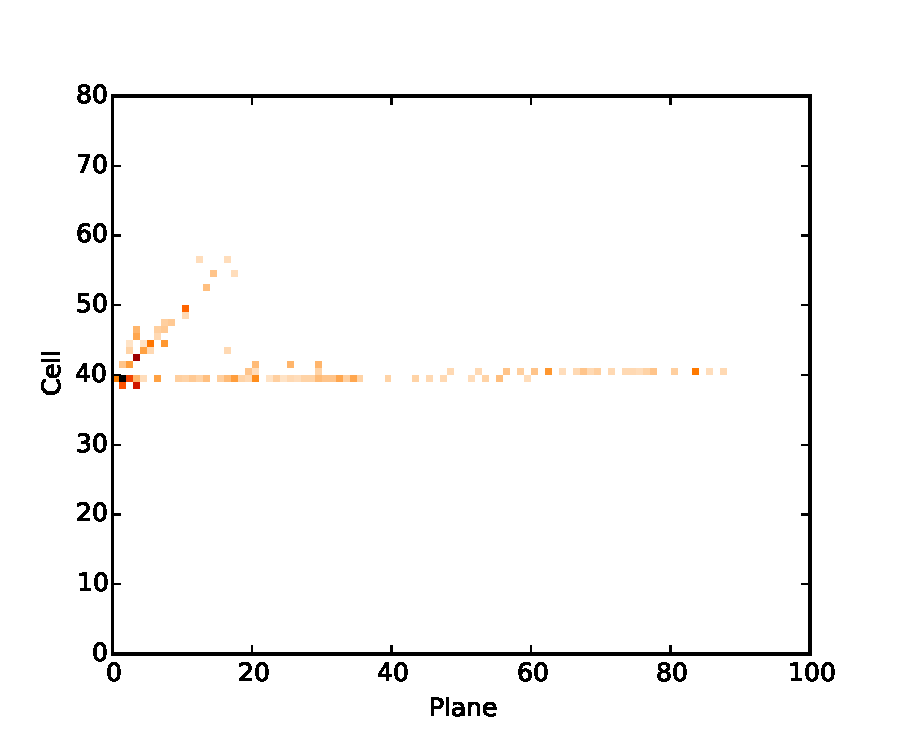
\includegraphics[width=\textwidth]{figures/cnn/view_truetype2_caltype2_event274_x.pdf}
\vspace{-20pt}
\caption*{\xview}
\end{subfigure}
\begin{subfigure}[c]{0.7\textwidth}
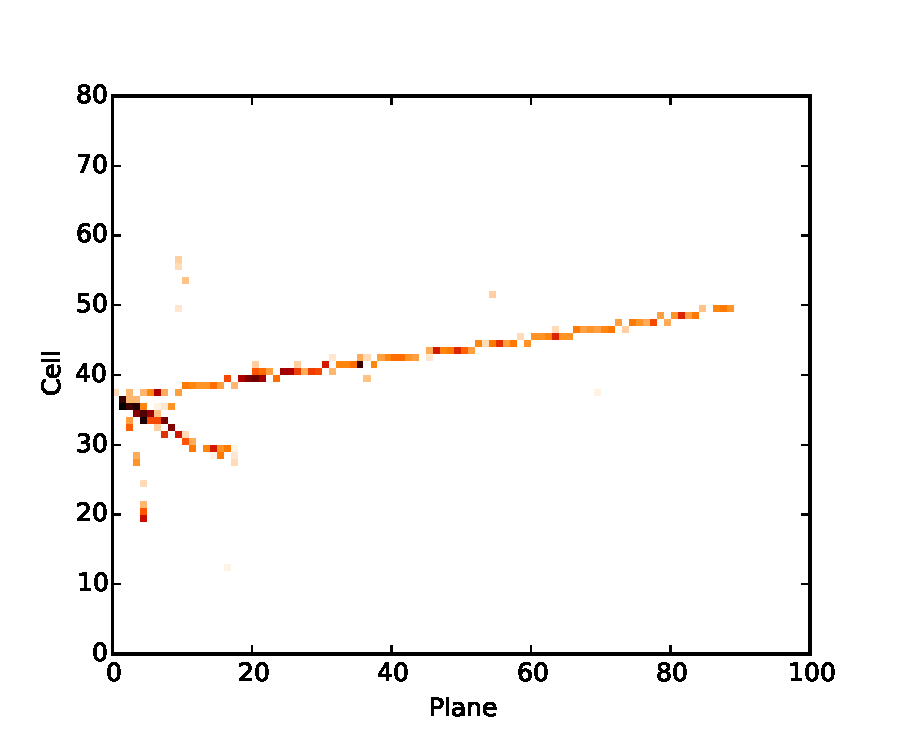
\includegraphics[width=\textwidth]{figures/cnn/view_truetype2_caltype2_event274_y.pdf}
\vspace{-20pt}
\caption*{\yview}
\end{subfigure}
\vspace{-10pt}
\end{center}
\caption{Image formed from a \numu CC interaction}{
Images such as this one are passed as input to the convolutional neural network.
The top and bottom panes show the \xview and \yview, respectively.
The region of interest is determined by the furthest plane upstream with
activity and the median cell position of all activity
in the 100 plane window spanned by the image.
The pixel intensity is proportional to the calibrated energy deposition
of each cell hit.
This particular image consists of a long muon track and a hadronic shower.}
\label{pixnumu}

\end{figure}

\begin{figure}
\begin{center}
\vspace{-40pt}
\begin{subfigure}[c]{0.7\textwidth}
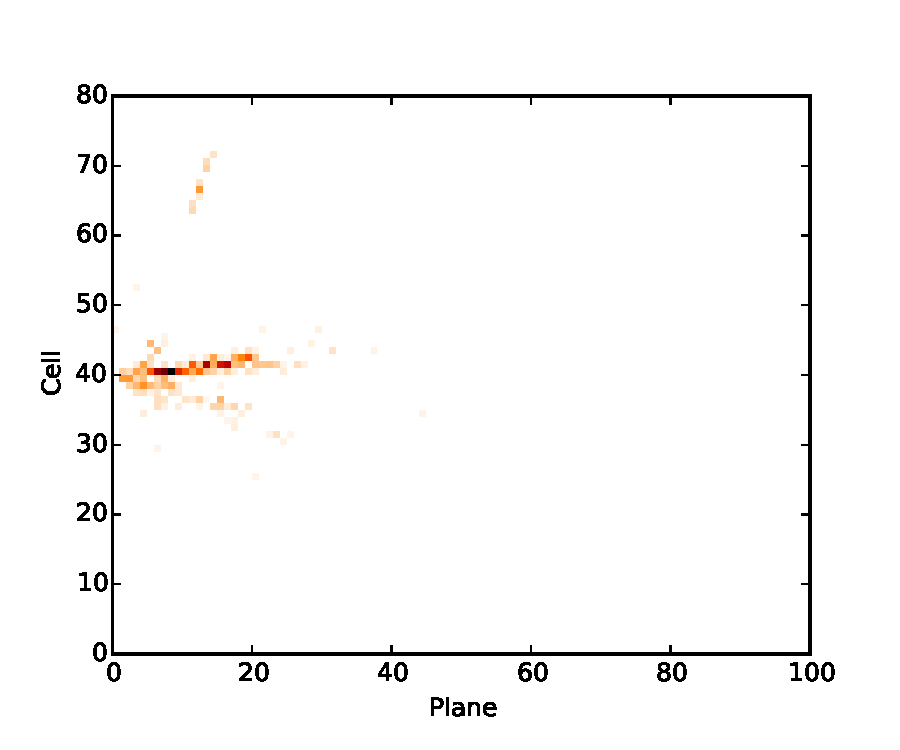
\includegraphics[width=\textwidth]{figures/cnn/view_truetype6_caltype6_event155_x.pdf}
\vspace{-20pt}
\caption*{\xview}
\end{subfigure}
\begin{subfigure}[c]{0.7\textwidth}
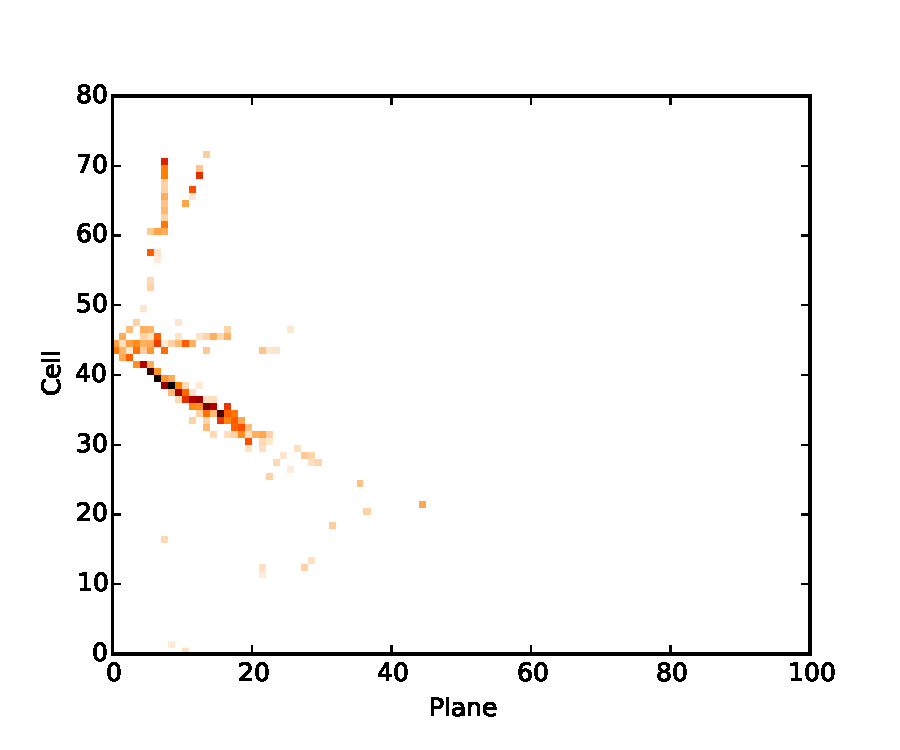
\includegraphics[width=\textwidth]{figures/cnn/view_truetype6_caltype6_event155_y.pdf}
\vspace{-20pt}
\caption*{\yview}
\end{subfigure}
\vspace{-10pt}
\end{center}
\caption{Image formed from a \nue CC interaction}{
Images such as this one are passed as input to the convolutional neural network.
The top and bottom panes show the \xview and \yview, respectively.
The region of interest is determined by the furthest plane upstream with
activity and the median cell position of all activity
in the 100 plane window spanned by the image.
The pixel intensity is proportional to the calibrated energy deposition
of each cell hit.
This particular image consists of a long muon track and a hadronic shower.}
\label{pixnue}

\end{figure}

\begin{figure}
\begin{center}
\vspace{-40pt}
\begin{subfigure}[c]{0.7\textwidth}
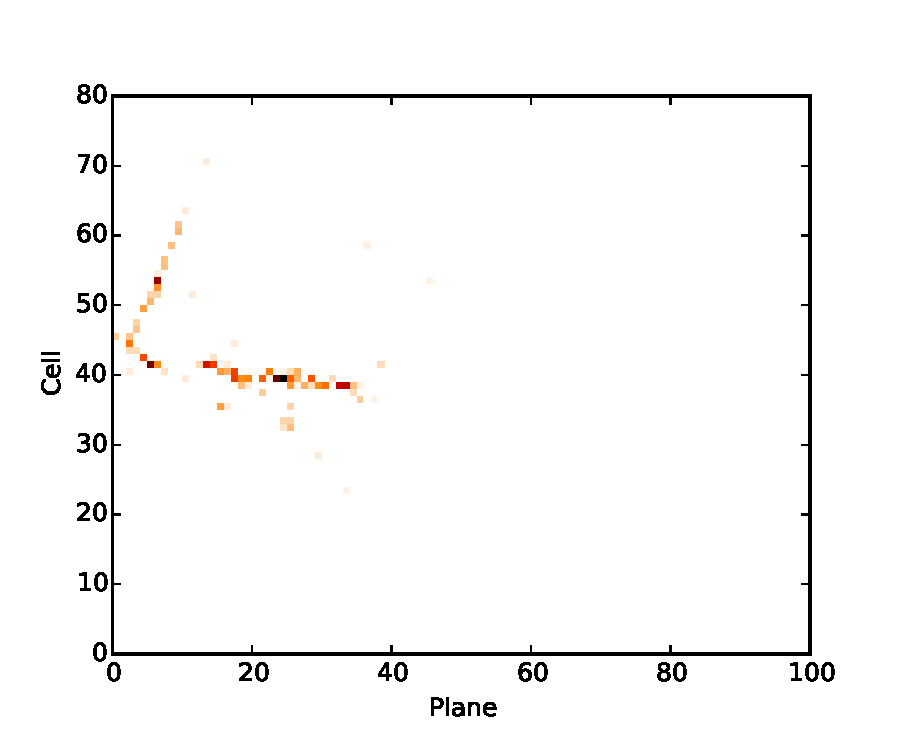
\includegraphics[width=\textwidth]{figures/cnn/view_truetype13_caltype6_event144_x.pdf}
\vspace{-20pt}
\caption*{\xview}
\end{subfigure}
\begin{subfigure}[c]{0.7\textwidth}
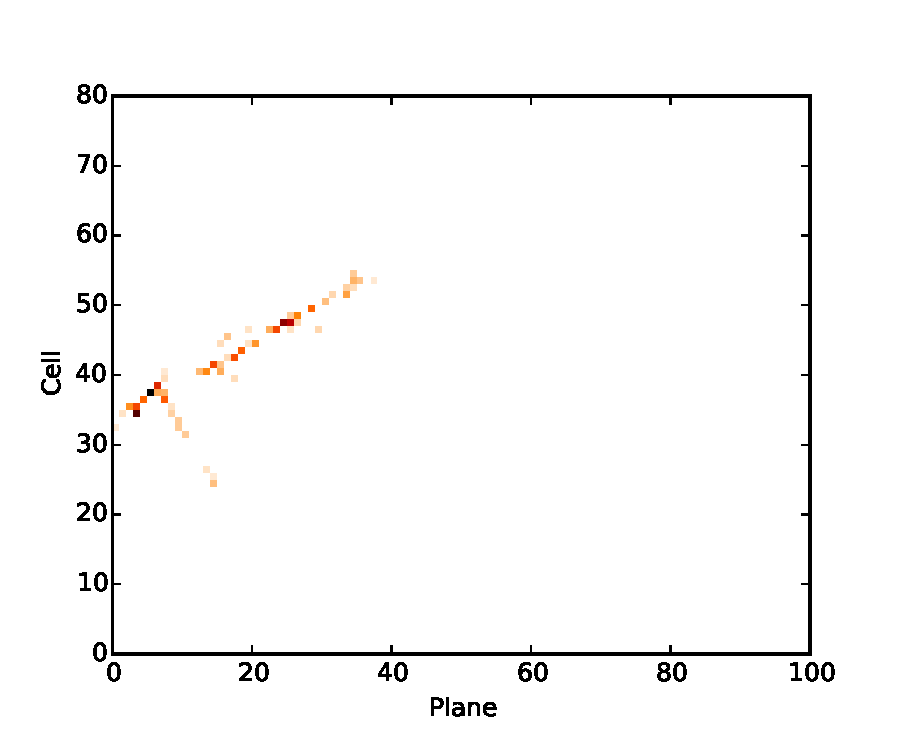
\includegraphics[width=\textwidth]{figures/cnn/view_truetype13_caltype6_event144_y.pdf}
\vspace{-20pt}
\caption*{\yview}
\end{subfigure}
\vspace{-10pt}
\end{center}
\caption{Image formed from an NC interaction}{
Images such as this one are passed as input to the convolutional neural network.
The top and bottom panes show the \xview and \yview, respectively.
The region of interest is determined by the furthest plane upstream with
activity and the median cell position of all activity
in the 100 plane window spanned by the image.
The pixel intensity is proportional to the calibrated energy deposition
of each cell hit.
This particular image consists of a hadronic shower including a neutral
pion which decays to two photons.}
\label{pixnc}
\end{figure}

Rather than using the readout of the entire detector, it is sensible to use
the reconstructed slices discussed in section \ref{slicer_section}.
The performance of DBSCAN in isolating cosmic rays and neutrino interactions
is robust and efficient enough \cite{baird2015thesis} that relying on this
simple reconstruction step will does significantly impact classification
results.
In the case of slices, the distance from the readout electronics is determined
by the mean position of all activity in the opposite view.

Each slice is transformed into an image by locating a region of interest to
capture activity.  The images are 80 cells wide and 100 cells deep in either
view.
The upstream side of the image is the first plane with a hit
in the slice.  In either view, the center of the image is defined by the
median cell position among all hits within the 100 plane window spanned by the
image.
The size and placement of this window ensures that the majority of beam events
are well contained, including \numu CC interactions which are
characteristically extensive as a result of long muon tracks.
Example images can be seen in Figures \ref{pixnumu}, \ref{pixnue},
and \ref{pixnc}.

\begin{figure}
\begin{center}
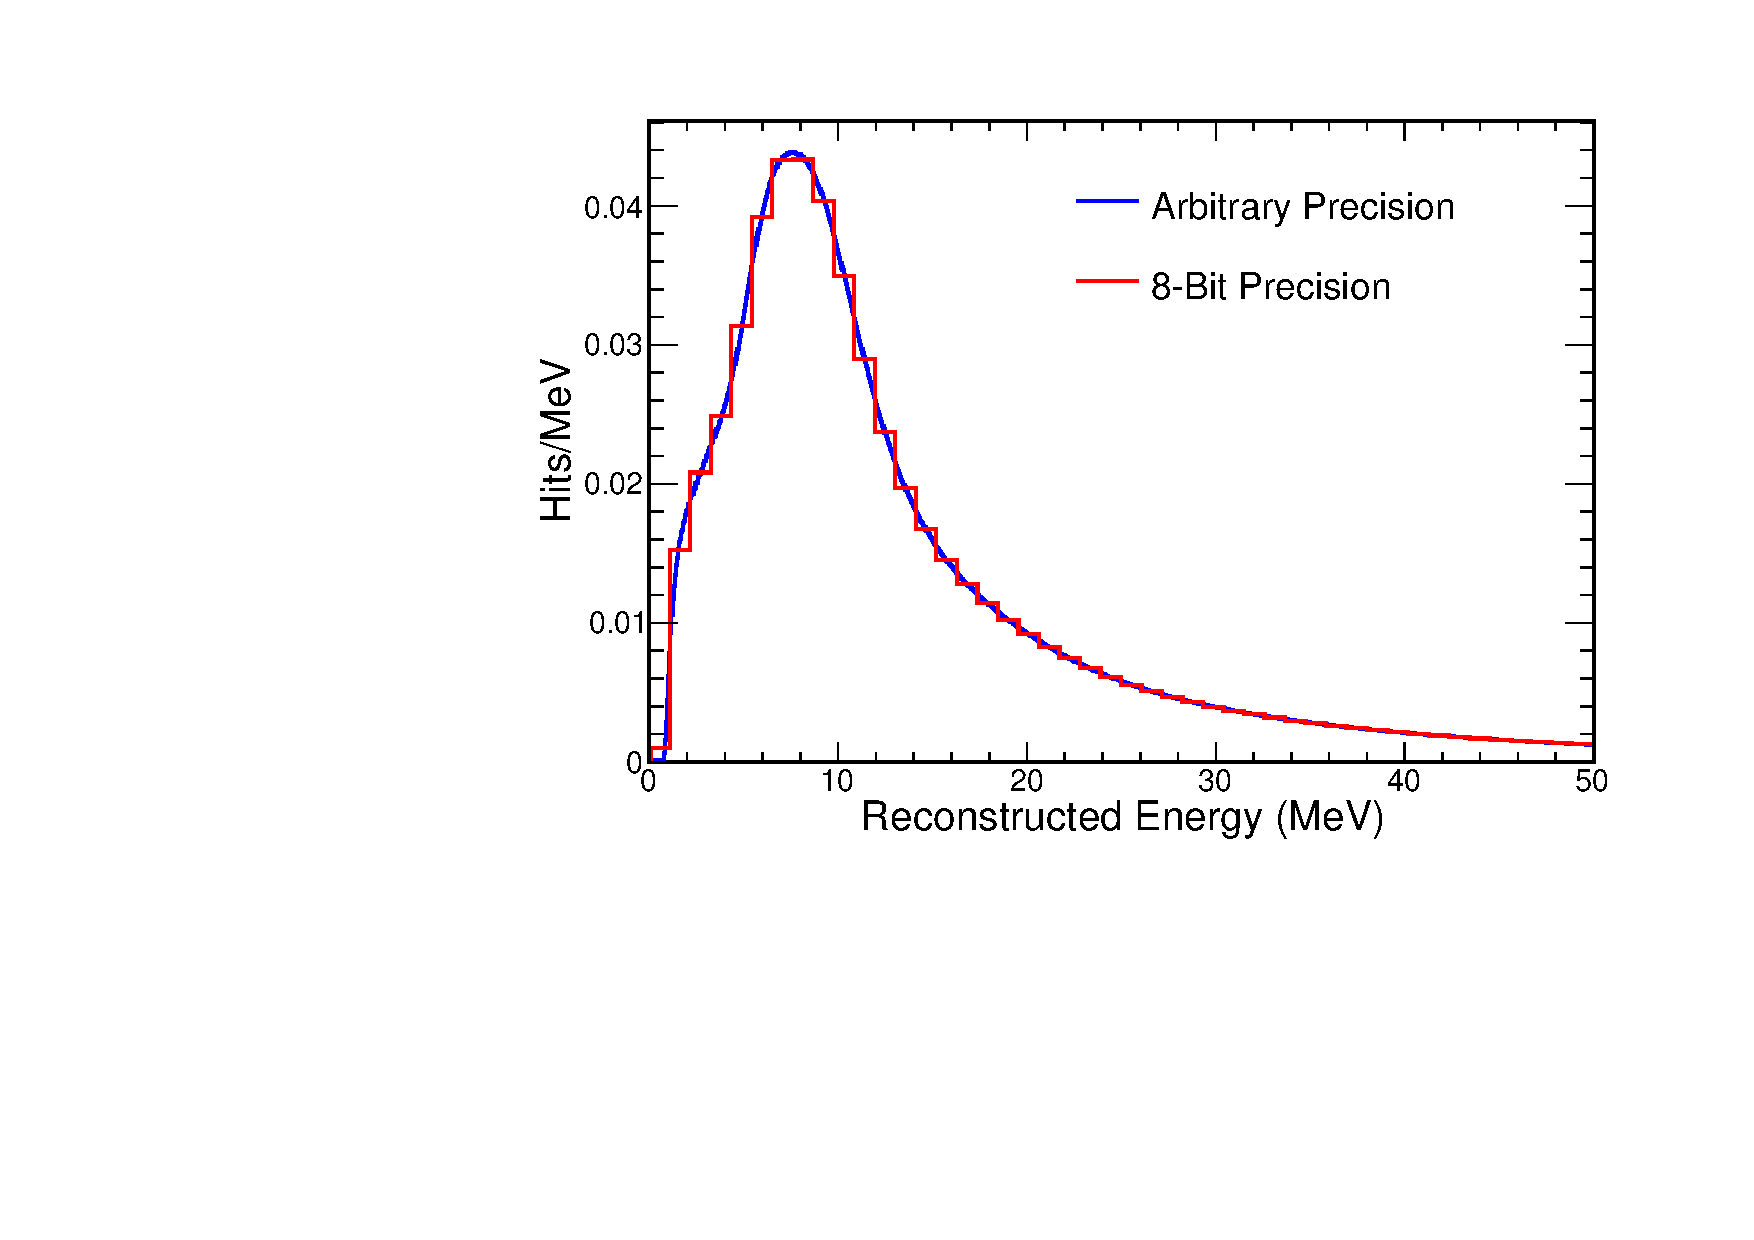
\includegraphics[width=0.85\textwidth]{figures/cnn/discrete_intensity.pdf}
\end{center}
\caption{Comparison of continuous hit intensity scale and discretized scale}{
Data volume is reduced by converting the continuous intensity scale of cell
hit energy depositions into a scale with 256 discrete values.
The discrete scale can be represented with eight bits, offering a significant
savings over a floating point representation.
}
\label{pixelmapadc}
\end{figure}


Pixel intensity in the image is proportional to the calibrated
energy deposition in each cell.
Images are thus interpretable as gray-scale with the shade of
each pixel corresponding to the amount of energy recorded in that cell.
In order to optimize data storage and transfer in the training stage,
the pixel intensities are converted to a scale of 256 discrete values
from the double precision floating point representation calibration result.
This conversion offers a factor of eight savings (eight bit versus 64 bit) in
savings over a floating point representation
without significantly compromising the representational capacity.
The importance of this savings is especially visible in reading data from
disk into memory during training.
A comparison original continuous scale and discrete scale can be seen in figure
\ref{pixelmapadc}.

\begin{figure}
\begin{center}
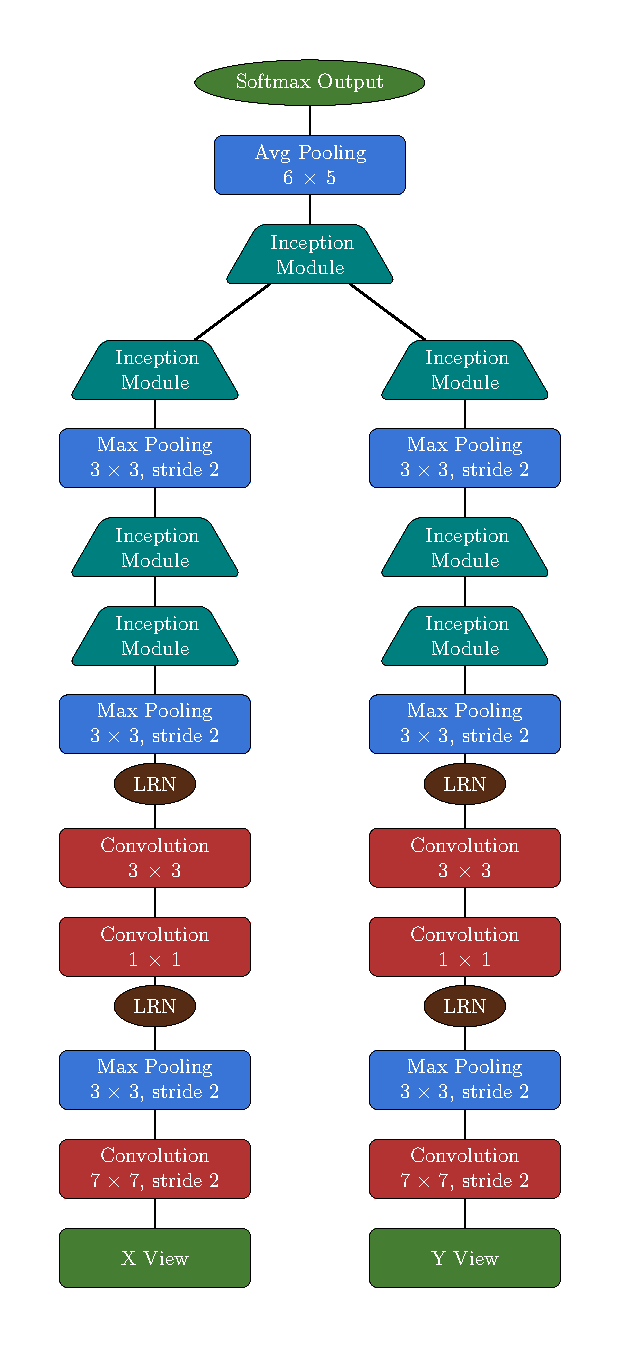
\includegraphics[height=0.8\textheight]{figures/arch/arch.pdf}
\end{center}
\caption{Diagram of the convolutional neural network architecture used
for event classification}{Starting with the input at the bottom,
the network has separate branches for the \xview and \yview.
Each branch undergoes successive convolution, pooling, and
local response normalization (LRN).  Inception modules are used in downstream layers.
The two views are merged and passed through a final inception module, and
pooled.  The output of the network comes from softmax units.
}
\label{arch}
\end{figure}


\section{Architecture}

The network architecture used in for this analysis is primarily based on
the \googlenet architecture \cite{szegedy2014going} introduced in section
\ref{googlenet_section}.
Initial experiments were performed with a full implementation of \googlenet
for each view, with only the final fully-connected layers merged.
It was observed during training, however,
that the classification of the second intermediate
loss unit showed equivalent classification accuracy to the final loss unit.
The architecture was then pruned and restructured in order to reduce
the total number of operations, and thus the amount of computation required
for training and evaluation.
No degradation was observed in the classification results with the pruned
architecture.
A depiction of the architecture can be seen in Figure \ref{arch}.

Input from the \xview and \yview is handled separately in two branches of the
network which are only merged in the final few layers.
Early in the network, images are subjected to $7\times7$ convolution and
$3\times3$ pooling, both with a stride of two.
Using stride two in these early layers scales the images down by a factor of
four.
Local response normalization (LRN) \cite{krizhevsky2012imagenet} is used
to smooth the filtered images.  Two more convolution operations, $1\times1$
and $3\times3$ are used, then another pass of smoothing with LRN, and
$3\times3$ pooling with stride two.  The $1\times1$ convolution serves
as dimensionality reduction in the number of filters.
A pair of inception modules is then used, then another $3\times3$ pooling layer
with stride two and another inception module.  The filter outputs for each view
are then concatenated and passed through another inception module.  A final
pass of average pooling is employed before a softmax layer, which serves as
the output of the network.


In the interest of time, the architecture presented here has only been coarsely
optimized, leaving plenty of room for further study.
It seems quite likely that a significantly more compact network could perform
equally as well.
Classification results could also perhaps be improved through fine tuning of
the architecture.
Eliminating the aggressive downsampling with stride two in the early layers
could significantly increase the level of detail which is available in the
inception modules.
Merging views earlier in the architecture could provide higher levels of
abstraction and greatly reduce the number of operations required.
The effect of LRN should be studied by removing those layers and
comparing results.


\section{Regularization}

A few regularization techniques were applied in order to enhance the ability
of the network to generalize beyond the training sample.
To keep the network weights small, weight decay term was included in the loss
function equal to $2\times 10^{-4}$ times the squared \textit{L2} norm of the
weight vector.
The softmax output layer was also subjected to dropout
\cite{hinton2014dropout}, described in section \ref{regularization_section},
with a probability of 0.4.

Perhaps the most robust defense against over training is more training
data.
In the absence of infinitely large and variegated training samples, however,
we can augment our sample by deliberately randomly changing the input image.
Two techniques were employed in order to add variation to the dataset.
First, Gaussian noise was applied to all pixel intensities with
a standard deviation of 1\%.
Since no Monte Carlo simulation is perfect, adding noise has the added benefit
of training the network to rely less heavily on the simulated intensity
in each pixel.
Second, events were randomly selected to be reflected in the cell dimension,
which is roughly transvese to the beam direction.
Symmetry about in the cell dimension is not perfect; the beam axis is directed
$3^{\circ}$ above detector horizon and attenuation in the optical fiber
causes thresholding to become more significant for hits further from
the readout electronics.
These effects are small, however, and their presence in fact aids in
enhancing variation of the training sample and deweighting precise details
of the Monte Carlo simulation.


\section{Training}

Training was performed using the Caffe framework \cite{jia2014caffe}
using NVIDIA Tesla K20 and K40 graphics processing units (GPU).
Weight updates were
performed using the basic stochastic gradient descent (SGD)
\cite{reed1999neural} procedure described in Chapter \ref{nnet_chapter}.

\begin{figure}
\begin{center}
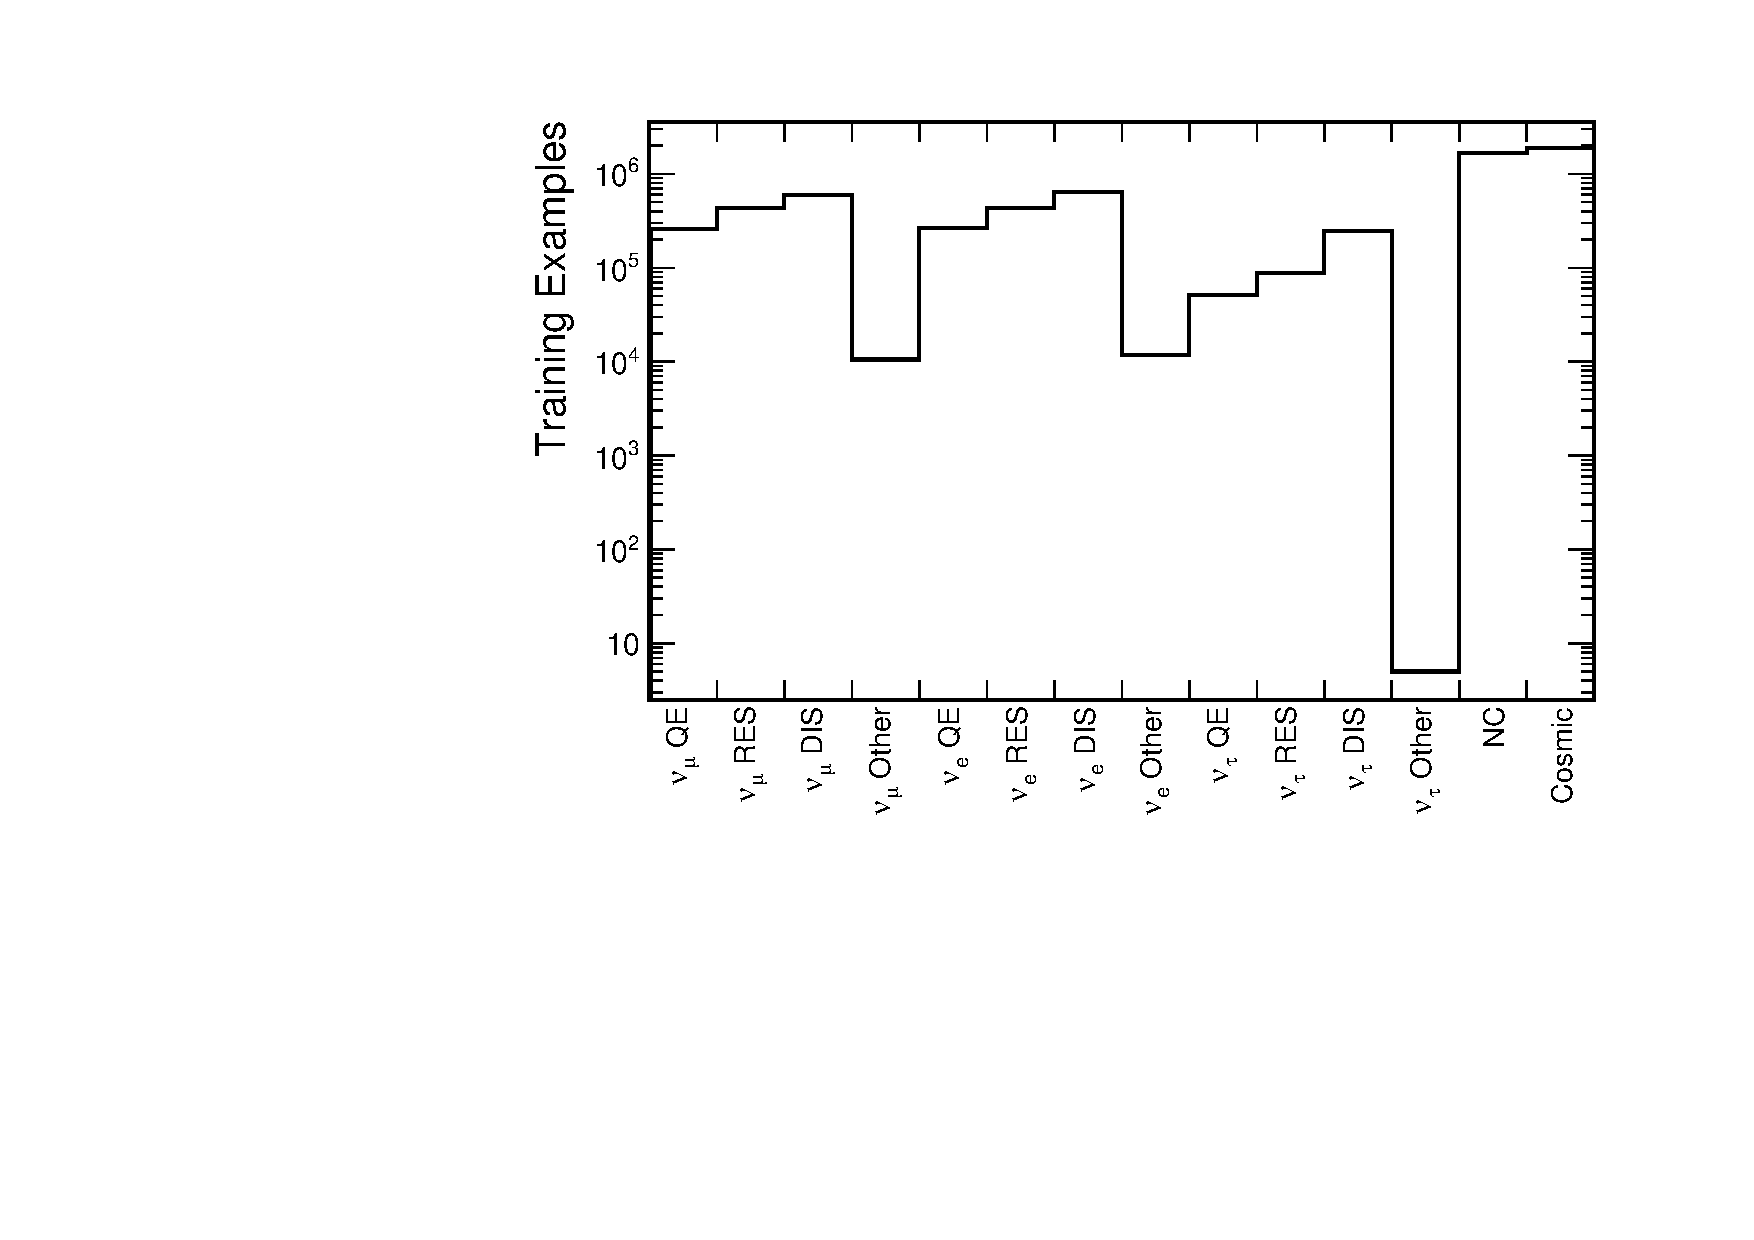
\includegraphics[width=\textwidth]{figures/cnn/traindist.pdf}
\end{center}
\caption{Histogram depicting class distribution for training dataset}{
  Training events are taken from \nova MC.  Events are simulated with the
  \numi energy spectrum and flavor distribution, ignoring oscillation.
  Samples of \nue and \nutau events are enhanced by respectively interchanging the \nue and \nutau components with the \numu components.
  Cosmic rays were only included in the sample during the fine-tuning phase of
  the training.
}
\label{traindist}
\end{figure}

The training sample was taken from \nova Monte Carlo simulation.
Events are simulated with an energy, interaction, flux distribution
corresponding to the \numi beam spectrum convoluted with \genie
cross section model.  Enhanced samples of \nue and \nutau
events are generated by respectively interchanging the \nue and \nutau
of the \numi beam flux with the vastly dominant \numu component.
Flavor interchange is based on the neutrino flux
upstream of \genie cross section convolution to allow proper interaction
weighting.
More details on the simulated neutrino spectrum can be found in section
\ref{genie_section}.
Cosmic ray data were added to the training sample for fine-tune training phase.
The events were required to pass a preselection based on track
containment and angle of the reconstructed track from the CosmicTrack algorithm
described in section \ref{cosmictrack_section}.
The cosmic ray preselection will be described in section
\ref{cosmicveto_section}.



Events were split into classes based on the interacting $\nu$ flavor and
\genie interaction mode.
NC interactions are grouped into a single class regardless of $\nu$ flavor.
For CC interactions, a class is formed for each flavor (\nue, \numu, \nutau)
and \genie interaction mode combination.
The QE, RES, and DIS modes each form their a distinct class, with
all other interactions placed in an ``other" category.
Separating events by interaction mode is motiated as an attempt to give
the network a hint at the underlying physics to aid in training.
Another class is reserved for cosmic rays.
In total, the training sample included 4.7 million neutrino events from \nova
simulation and 1.8 million events from cosmic ray data.
The class distribution can be seen in table \ref{traindist_table} and
visualized as a histogram in table \ref{traindist}.




Due to GPU memory constraints, a mini-batch training scheme was employed.
In mini-batch training, gradients used in weight updates are averaged over
small sub-samples of the training dataset rather than the entire sample.
After calculating the gradient for a batch, it is flushed from memory
and the next batch is loaded.
Batches are reused after each full pass over the training dataset
A batch size of 32 was used to train the network.
Each pass over a mini-batch is referred to as an \textit{iteration};
a full pass over the dataset is called an \textit{epoch}.



\begin{table}
\begin{center}
\begin{tabular}[t]{|c|c|c|}
\hline
\multicolumn{2}{|c|}{\textbf{Class Label}} &
\textbf{Number of Training Examples} \\ \hline
\multirow{4}{*}{\numu}  & QE &  261,823 \\ \cline{2-3}
 & RES &  429,470 \\ \cline{2-3}
 & DIS &  601,497 \\ \cline{2-3}
 & Other &  10,546 \\ \hline
\multirow{4}{*}{\nue}  & QE &  266,111 \\ \cline{2-3}
 & RES &  434,720 \\ \cline{2-3}
 & DIS &  641,813 \\ \cline{2-3}
 & Other &  11,829 \\ \hline
\multirow{4}{*}{\nutau} & QE &  51,372 \\ \cline{2-3}
 & RES &  88,185 \\ \cline{2-3}
 & DIS &  248,408 \\ \cline{2-3}
 & Other & 5 \\ \hline
\multicolumn{2}{|c|}{NC} & 1,683,050 \\ \hline
\multicolumn{2}{|c|}{Cosmic Ray}  & 1,872,258 \\ \hline
\end{tabular}
\end{center}
\caption{Class distribution for training dataset}{
  Training events are taken from \nova MC.  Events are simulated with the
  \numi energy spectrum and flavor distribution, ignoring oscillation.
  Samples of \nue and \nutau events are enhanced by respectively interchanging the \nue and \nutau components with the \numu components.
  Cosmic rays were only included in the sample during the fine-tuning phase of
  the training.
}
\label{traindist_table}
\end{table}

The initial learning rate for SGD was set to 0.01.
During the training, the learning rate was decreased by a factor of 0.96
according to a prescribed schedule.
The learning rate was decreased after the first 100,000 iterations, again
after the next two sets of 50,000 iterations, then again after four sets of
25,000 iterations, and subsequently after each 10,000
iterations.

Training was interrupted after 640,000 iterations after an error
was discovered in the architecture.
Rather than having the intended 15 nodes in the softmax output layer,
the architecture had accidentally been configured with 1,000 nodes in that
layer.
The architecture was modified to have the correct number of nodes, and training
was resumed by reloading trained weights from all layers but the output.
This method for resolving the error was justified by an approach
commonly used for image classification competitions known as
\textit{fine-tuning} \cite{krizhevsky2012imagenet}.
Since learning occurs much more quickly in downstream layers relative to
upstream filters, downstream layers can be quickly fine-tuned based on
filters which have been trained in advance.
Upon resuming training, the learning rate was set to 0.002, roughly equal to
the learning rate reached after 640,000 iterations.
The decrease schedule, however, was started from the beginning rather
than reverting to the once every 10,000 iteration schedule
that would have been employed beyond iteration 640,000.

After 970,000 total iterations, the cosmic ray data were added to the
training sample.
With this enhanced training sample, the network was trained for another
990,000 iterations.
A separate version of the network was trained for 990,000 iterations
using cosmic ray data from the beginning, but was outperformed by the
other network in terms of overall accuracy.
In particular, the network originally trained on a beam-only training set
allowed for more pure \nue CC selection.


\section{Training Results}

\begin{figure}
\begin{center}
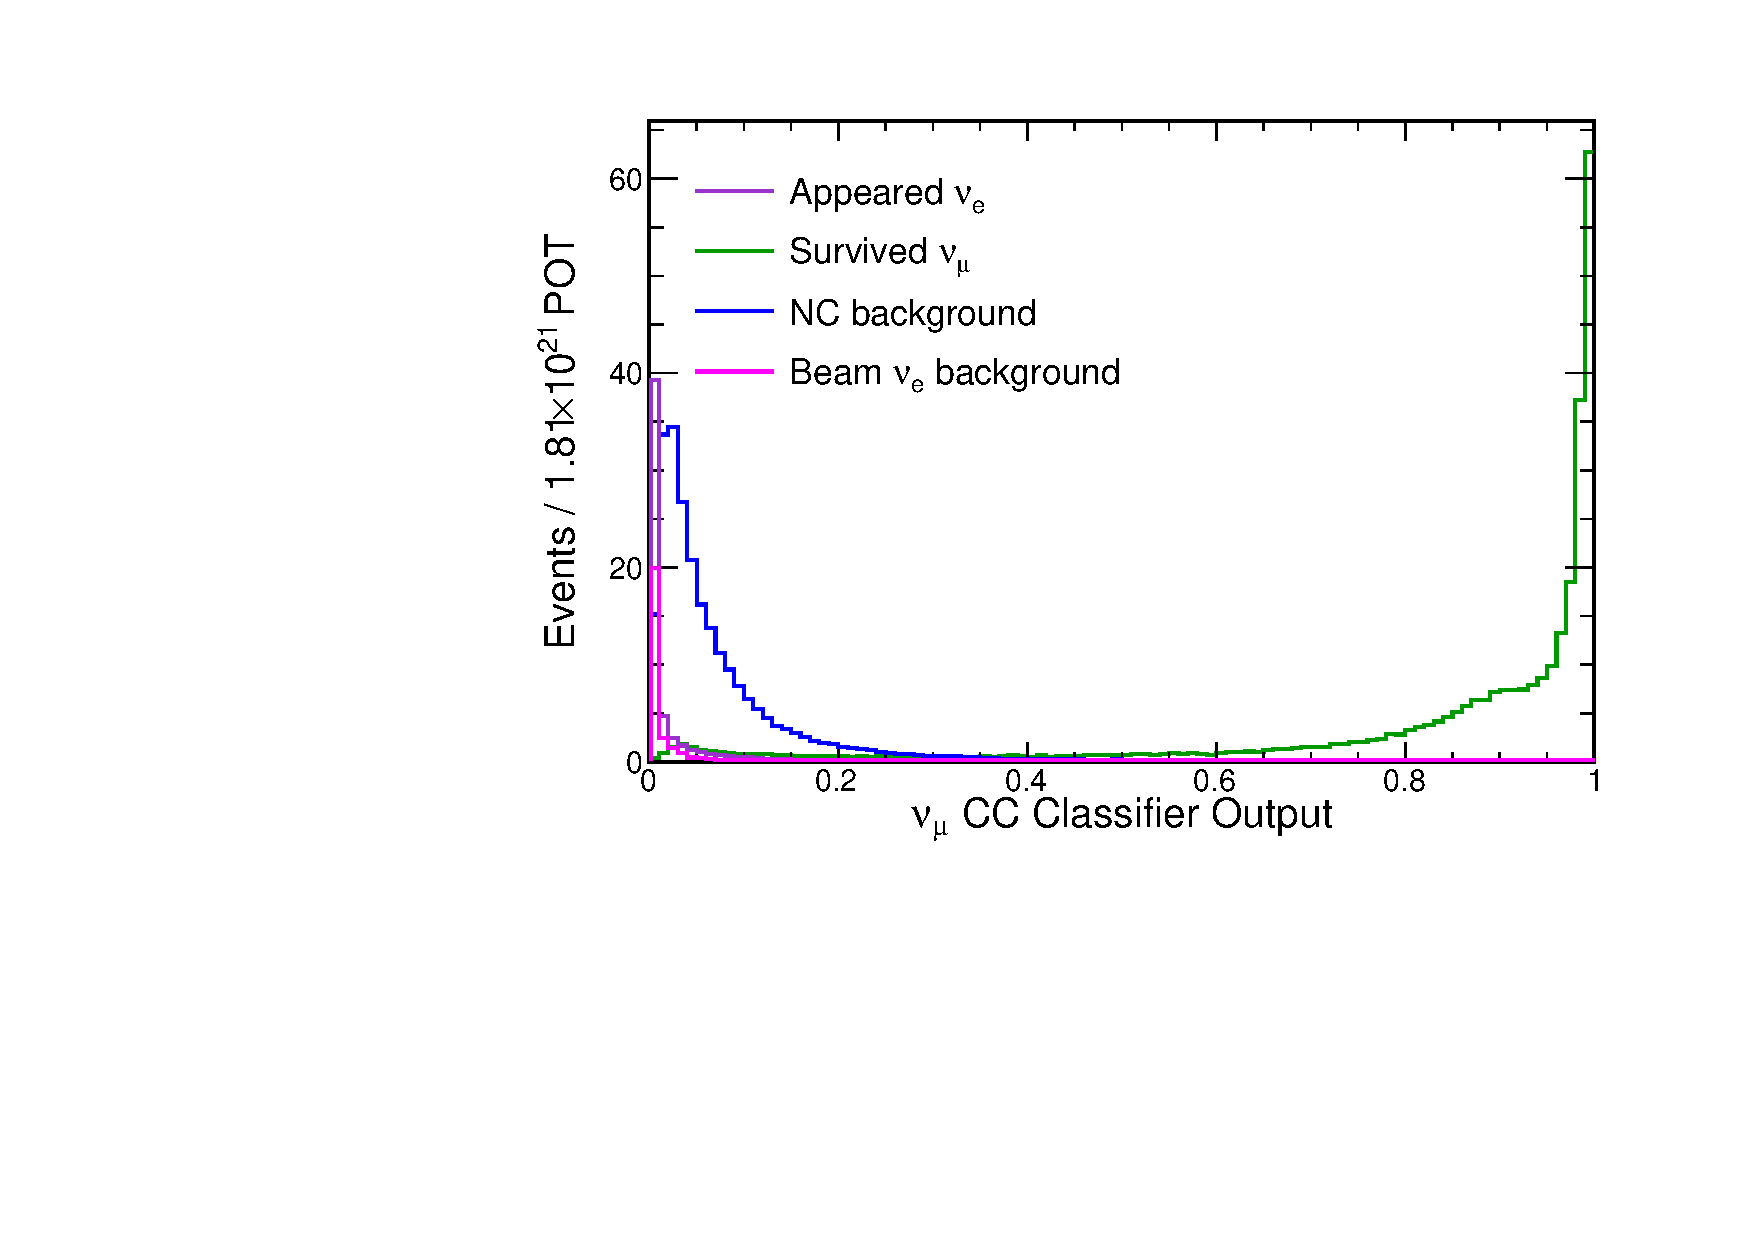
\includegraphics[width=0.85\textwidth]{figures/cnn/numu_pid_dist.pdf}
\end{center}
\caption{Histogram of the \nue classifier output}{
The survived \numu signal can be seen as as strong peak at the right.
Both \nue, and NC interactions all enter as a background
in \numu disappearance analysis.
Clear separation in the classifier can be seen between the signal and backgrounds.
}
\label{numupid}
\end{figure}


\begin{figure}
\begin{center}
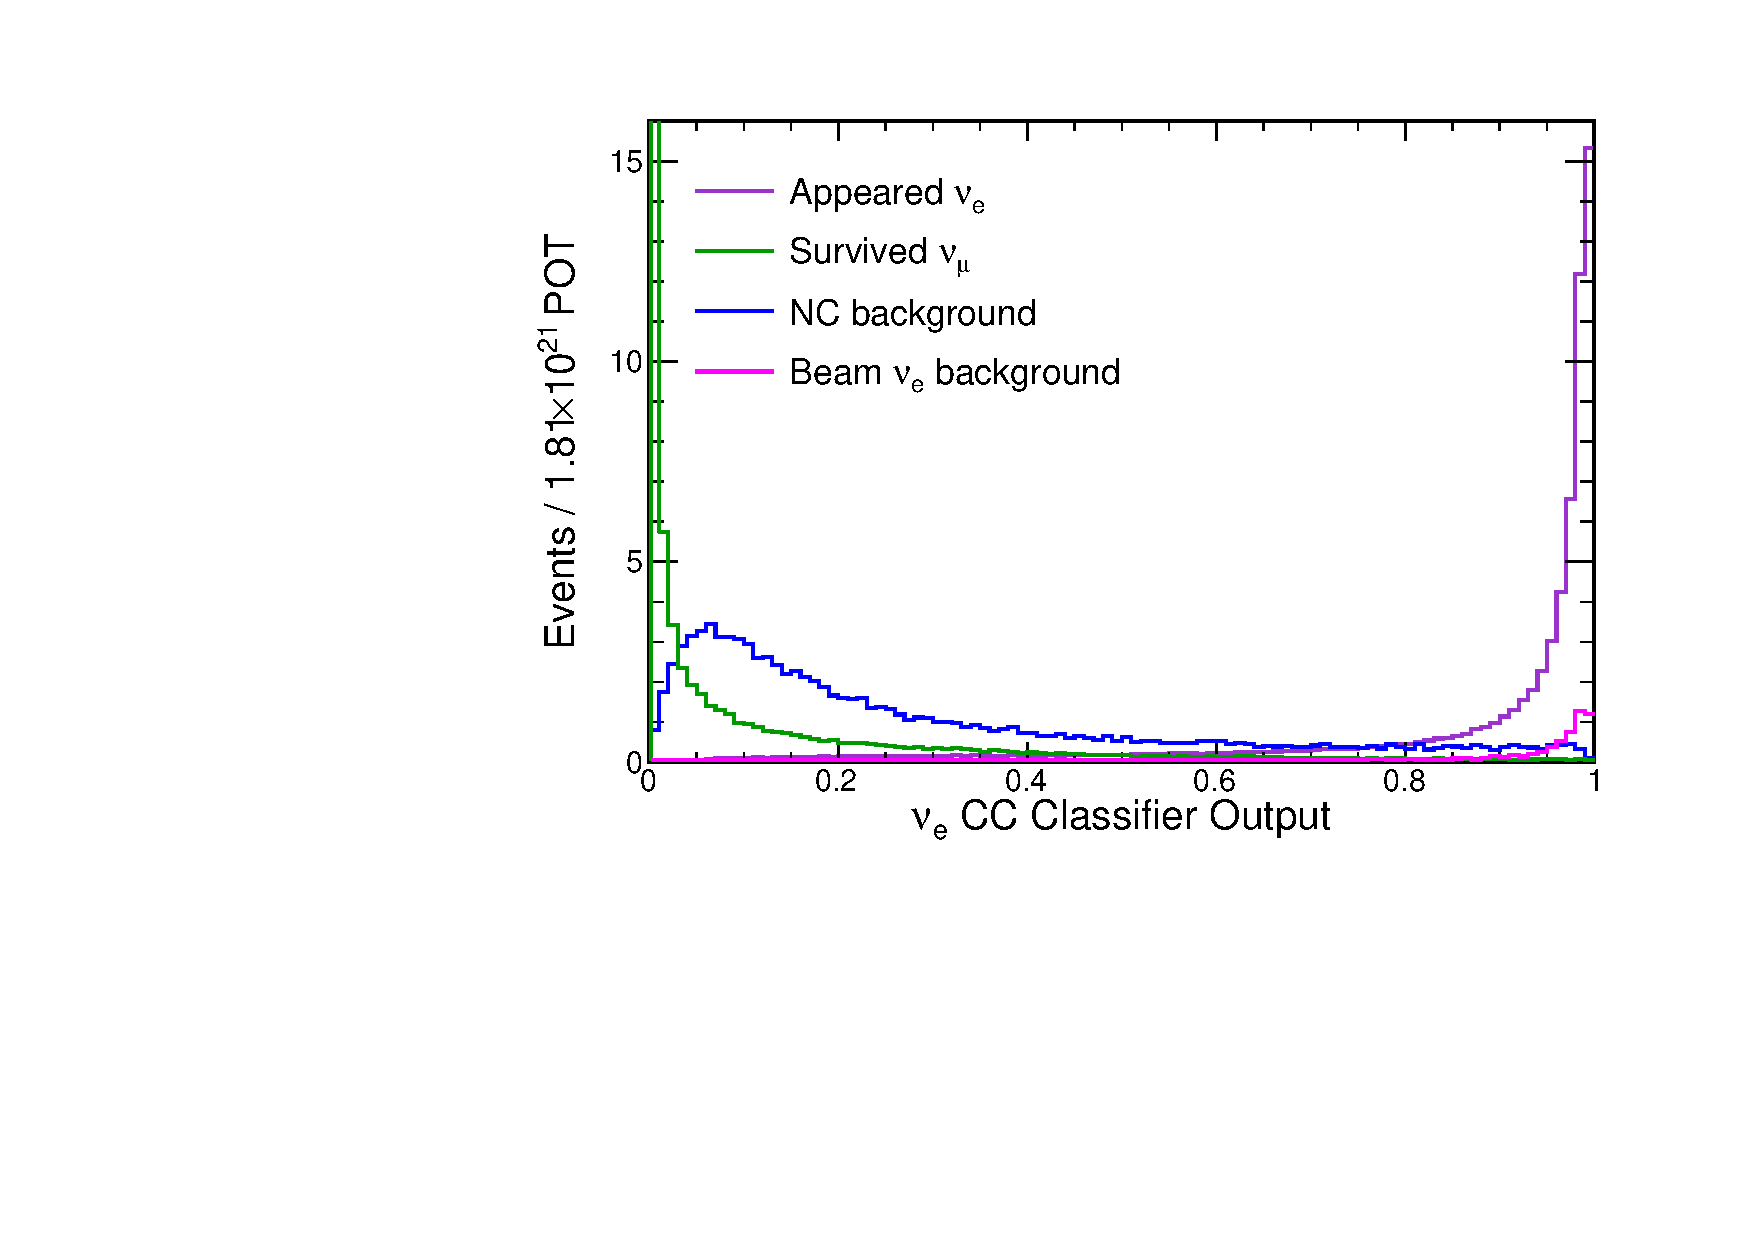
\includegraphics[width=0.85\textwidth]{figures/cnn/nue_pid_dist.pdf}
\end{center}
\caption{Histogram of the \numu classifier output}{
The appeared \nue signal can be seen as as strong peak at the right.
Survived \numu, beam \nue, and NC interactions all enter as a background
in \nue appearance analysis.
Clear separation in the classifier can be seen between the signal and backgrounds.
}
\label{nuepid}
\end{figure}


The trained network serves as a good classifier for $\nu$ oscillation analysis
involving both \numu disappearance and \nue appearance.
Classifier outputs \nue, \numu, and \nutau are formed by summing across the
softmax outputs for QE, RES, DIS, and Other subclasses.
The performance of this classifier has been demonstrated to outperform
all other classification approaches developed for the \nova oscillation
analyses.
The \numu and \nue classifier outputs can be seen in figures \ref{numupid} and
\ref{nuepid} respectively.
The application to \numu disappearance will be discussed in detail throughout
the rest of this thesis.


\section{Filter Visualization}

Since convolution and pooling layers preserve the spatial orientation of
information within an image, visualizing filters and filter output for
particular images can provide insight with regard to the network operation.
As observed in many convolutional neural network examples,
early layers in the network respond to low-level characteristics
in an image \cite{lecun2015deep}.
The $7\times7$ convolutional filters trained in the first layer can be seen
in Figure \ref{7x7conv}.
The output of those filters can be seen in Figures \ref{7x7numu}, \ref{7x7nue},
and \ref{7x7nc}.
Downstream layers in the network start to pick up higher level concepts,
like the presence of track-like or shower-like activity.
Output from the first inception module in the \yview branch can be seen
in Figure \ref{inceptionexamples}.



\begin{figure}
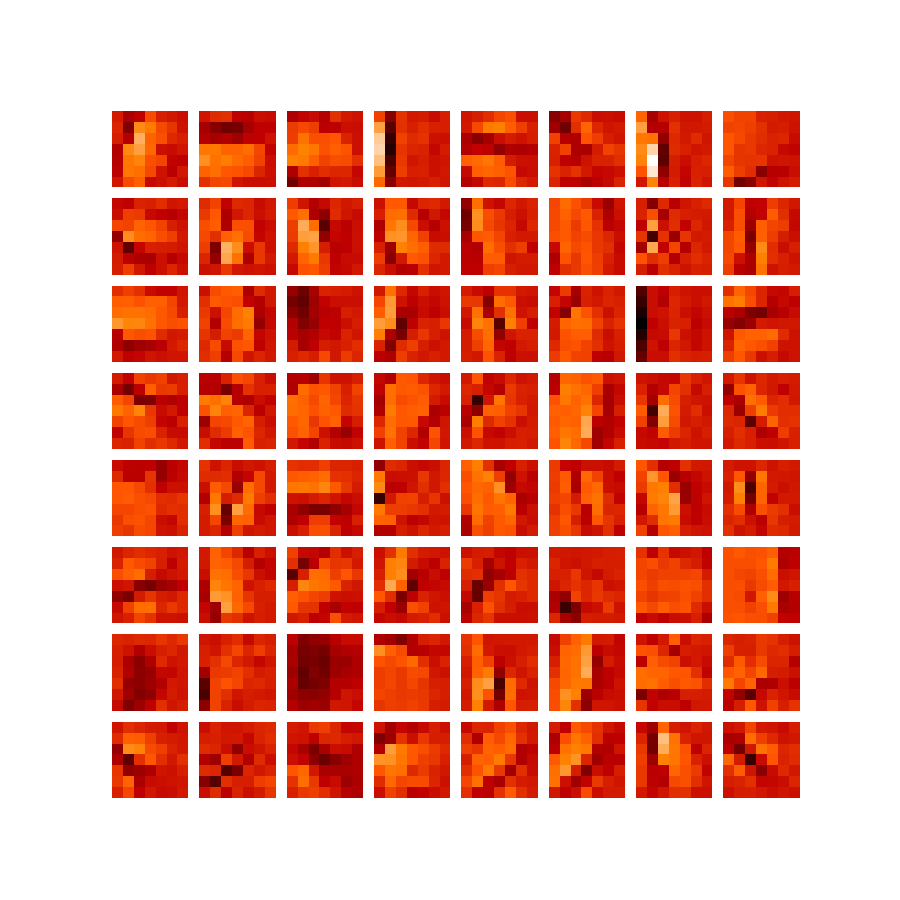
\includegraphics[width=\textwidth]{figures/cnn/conv1y.pdf}
\caption{$7\times7$ Convolutional Filters}{
The first layer of the network used for classification performs 64 different
$7\times7$ convolution operations for both the \xview and \yview.
Each entry in the grid above shows one of those trained filters from the
first layer of the \yview branch of the network.
}
\label{7x7conv}
\end{figure}

\begin{figure}
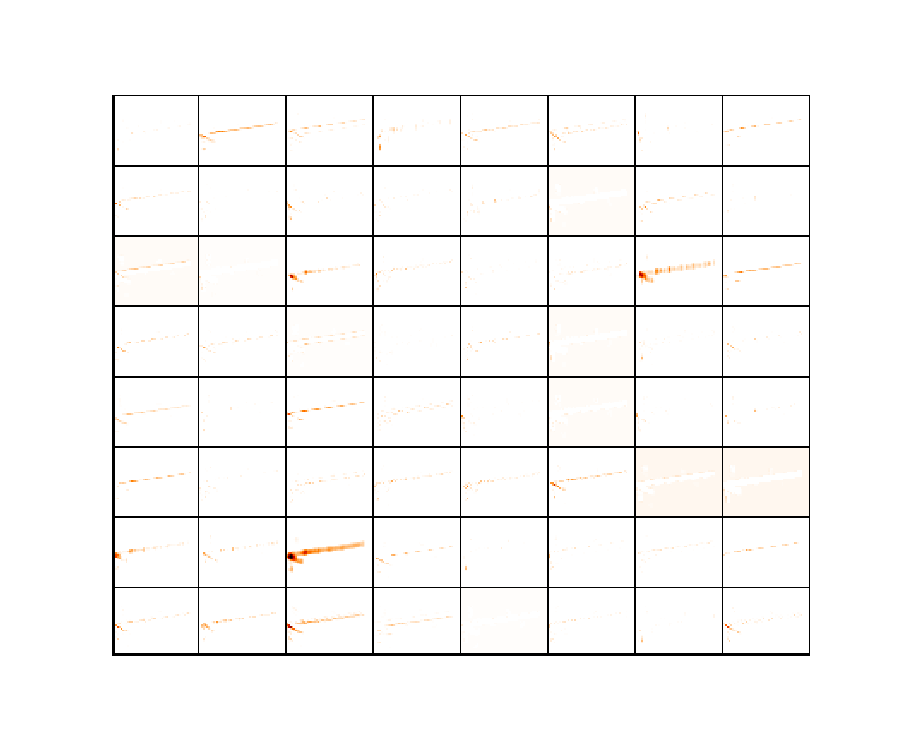
\includegraphics[width=\textwidth]{figures/cnn/feat1_truetype2_caltype2_event274_y.pdf}
\caption{$7\times7$ convolutional filter outputs for a \numu CC event}{
Convolutional filters produce many alternative representations of an image.
Each entry in the grid shows the the output in the corresponding location
of the grid in figure \ref{7x7conv}.
The input image for these filtered representations was the \yview image
of the \numu CC event from Figure \ref{pixnumu}
}
\label{7x7numu}
\end{figure}


\begin{figure}
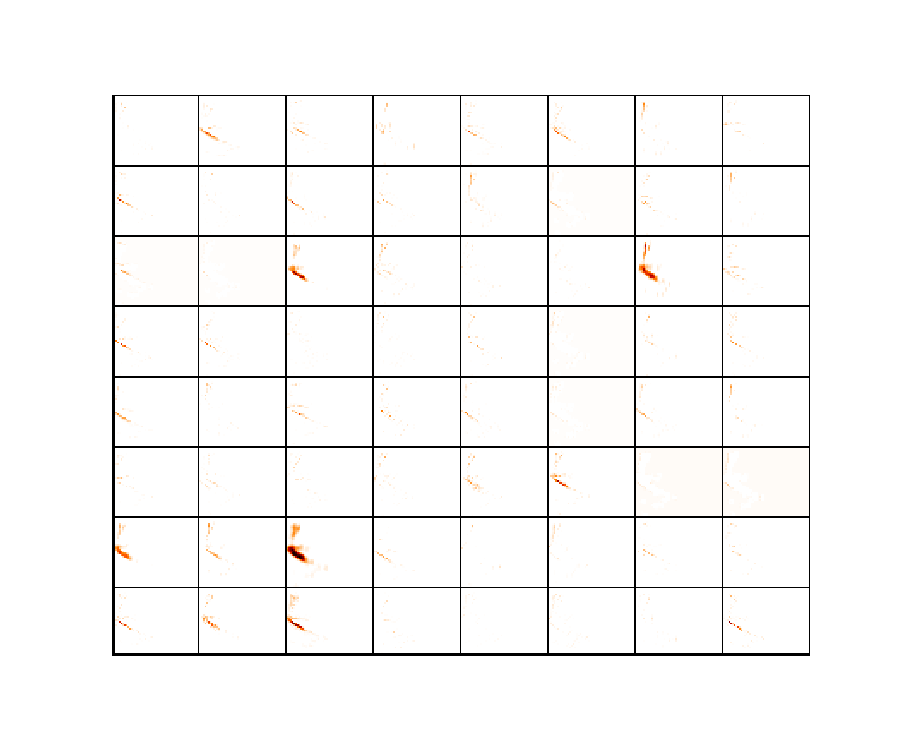
\includegraphics[width=\textwidth]{figures/cnn/feat1_truetype6_caltype6_event155_y.pdf}
\caption{$7\times7$ convolutional filter outputs for a \nue CC event}{
Convolutional filters produce many alternative representations of an image.
Each entry in the grid shows the the output in the corresponding location
of the grid in figure \ref{7x7conv}.
The input image for these filtered representations was the \yview image
of the \nue CC event from Figure \ref{pixnue}
}
\label{7x7nue}
\end{figure}


\begin{figure}
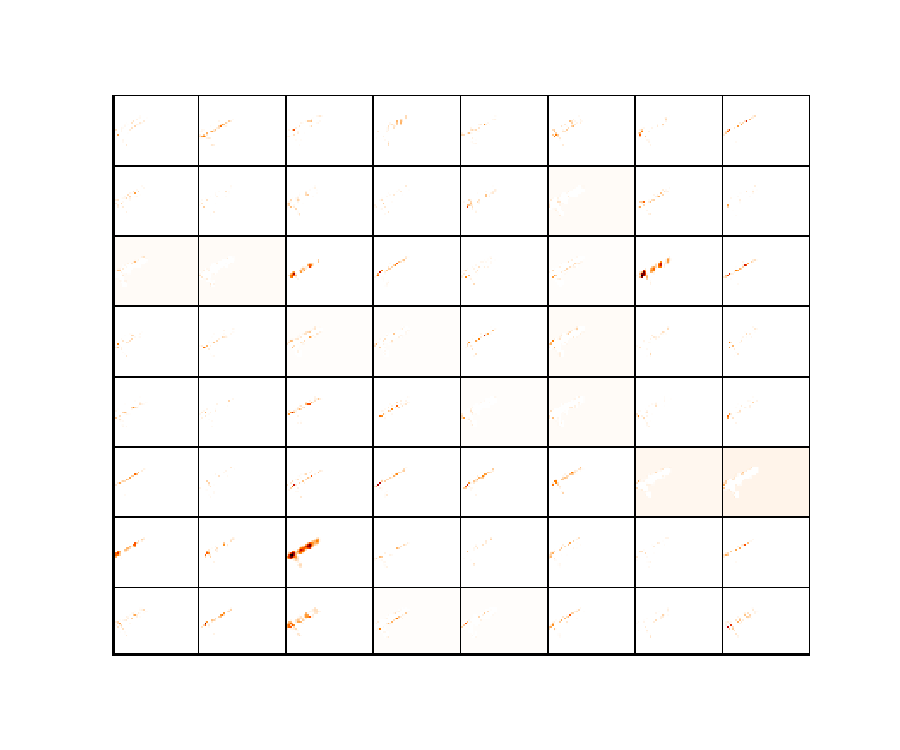
\includegraphics[width=\textwidth]{figures/cnn/feat1_truetype13_caltype6_event144_y.pdf}
\caption{$7\times7$ convolutional filter outputs for an NC event}{
Convolutional filters produce many alternative representations of an image.
Each entry in the grid shows the the output in the corresponding location
of the grid in figure \ref{7x7conv}.
The input image for these filtered representations was the \yview image
of the NC event from Figure \ref{pixnc}
}
\label{7x7nc}
\end{figure}



\begin{figure}
  \vspace{-25pt}
  \begin{center}
  \begin{subfigure}[b]{\textwidth}
    \centering
    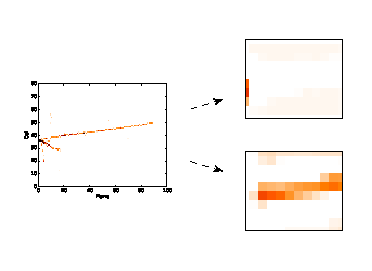
\includegraphics[width=0.58\textwidth,viewport=10 13 170 115, clip=true]{figures/cnn/featurePlotNuMuDIS}
    \caption*{\numu CC DIS event with with significant hadronic activity}
  \end{subfigure}%

  \begin{subfigure}[b]{\textwidth}
    \centering
    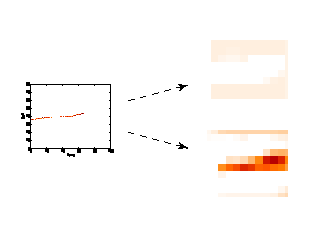
\includegraphics[width=0.58\textwidth,viewport=10 13 170 115, clip=true]{figures/cnn/featurePlotNuMuQE}
    \caption*{\numu CC QE event with with little hadronic activity}

  \end{subfigure}%

  \begin{subfigure}[b]{\textwidth}
    \centering
    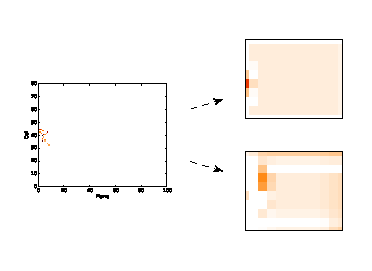
\includegraphics[width=0.58\textwidth,viewport=10 13 170 115, clip=true]{figures/cnn/featurePlotNC}
    \caption*{NC event with with solely hadronic activity}

  \end{subfigure}%
\end{center}
  \caption{Inception module filter output}
  {
    Input images and corresponding filter output from two particular
    filters in the first inception module in the \yview branch of the
    network.
    In each pane, the input image at left and filter outputs are at right.
    The top filter in each pane appears to responding to hadronic activity,
    while the bottom filter appears to correspond to more track-like activity.

  }
  \label{inceptionexamples}
\end{figure}


%%%%%%%%%%%%%%%%%%%%%%%%%%%%%%%%%%%%%%%%%%%%%%%%%%%%%%%%%%%%%%%%%%%%%%%%%%%%%%%%
